In Section~\ref{sec:language:key_value}, we have presented an algorithm for
replacing a key's value in a BST dictionary. To make the program more
interesting, we consider a sequence of $n$ lookup or replace operations for
different keys in the BST (which may or may not be repeated). A single lookup or
replace has worst-case time complexity $\mathcal{O}(h)$ where $h$ is the height
of the BST, therefore performing $n$ operations takes $\mathcal{O}(h \times n)$
time.

In order to reduce the execution time of the new program, we can cache the
search and replace operations so that repeated operations become faster. Instead
of traversing the entire height of the BST, we look in the cache and send the
operation immediately to the node where the key is located. Without thread
facts, we might have cached the results at the root node, however, this is not a
scalable approach as it would introduce a serious bottleneck.

Figure~\ref{code:threads:btree_lookup_cache} shows the updated BST code with a thread
cache. We just added two more predicates, \code{cache} and
\code{cache-size}, that are facts placed in the thread and represent cached
keys and the total size of the cache, respectively. We also added three new
rules that handle the following cases:

\begin{enumerate}
      \item A key is found and is also in the cache
         (lines~\ref{line:threads:kv_rule1_start}-\ref{line:threads:kv_rule2_end}
         in Fig.~\ref{code:threads:btree_lookup_cache});

      \item A key is found but is not in the cache
         (lines~\ref{line:threads:kv_rule2_start}-\ref{line:threads:kv_rule2_end}
         in Fig.~\ref{code:threads:btree_lookup_cache});

      \item A key is in the cache, therefore a \code{replace} fact is
         derived in the target node
         (lines~\ref{line:threads:kv_rule3_start}-\ref{line:threads:kv_rule3_end}).

\end{enumerate}

Note that it is quite easy to extend the cache mechanism to use an LRU type
approach in order to limit the size of the cache.

\begin{figure}[ht]
\begin{Verbatim}[numbers=left,fontsize=\codesize,commandchars=*\{\}]
type left(node, node).*hfill// Predicate declaration
type right(node, node).
type linear value(node, int Key, string Value).
type linear replace(node, int Key, string Value).
type linear cache(thread, node, int).
type linear cache-size(thread, int).

replace(A, Key, RValue),*hfill*label{line:threads:kv_rule1_start}// Rule 1: key exists and is also in the cache
value(A, Key, Value),
*underline{cache(T, A, Key)}
   -o value(A, Key, RValue).
      *underline{cache(T, A, Key)}.*label{line:threads:kv_rule1_end}

replace(A, Key, RValue),*label{line:threads:kv_rule2_start}*hfill// Rule 2: key exists and is not in the cache
value(A, Key, Value),
*underline{cache-size(T, Total)}
   -o value(A, Key, RValue),
      *underline{cache-size(T, Total + 1)},
      *underline{cache(T, A, Key)}.*label{line:threads:kv_rule2_end}

replace(A, RKey, RValue),*label{line:threads:kv_rule3_start}*hfill// Rule 3: cached by the thread
*underline{cache(T, TargetNode, RKey)}
   -o replace(TargetNode, RKey, RValue),
      *underline{cache(T, TargetNode, RKey)}.*label{line:threads:kv_rule3_end}

replace(A, RKey, RValue),*hfill// Rule 4: go left
value(A, Key, Value),
!left(A, B),
RKey < Key
   -o value(A, Key, Value),
      replace(B, RKey, RValue).

replace(A, RKey, RValue),*hfill// Rule 5: go right
value(A, Key, Value),
!right(A, B),
RKey > Key
   -o value(A, Key, Value),
      replace(B, RKey, RValue).
\end{Verbatim}
\caption{LM program for performing lookups in a BST extended to use a thread cache.}
\label{code:threads:btree_lookup_cache}
\end{figure}

In order to understand the effectiveness of the new cached version of the
program, we created synthetic datasets that stress the algorithm using a
complete binary search tree and an arbitrary number of (repeated) tree
operations such as replace and lookup. The tree operations apply to a subset of
the tree and each node is associated with a list of operations that need to be
performed. We have auxiliar nodes (not connected to the tree) that coordinate
the tree operations for a given node. An auxiliary node will start the first
operation by sending it to the tree root node. Once the operation is performed
on the target node, the auxiliary node will start the next operation in the list
for that target node. By using auxiliary nodes, we are able to experiment with a
operations that target the same node and also allow for some parallelism when
doing tree operations. In our experiments, we generated two trees with the
following characteristics:

\begin{itemize}
   \item 19 levels: a tree with 19 levels ($2^{20}-1$ nodes) and two million
      operations. Each targeted node has, on average, 40 operations.

   \item 21 levels: a tree with 21 levels ($2^{22}-1$ nodes) and five million
      operations. Each targeted node has, on average, 20 operations.
\end{itemize}

Note that in both datasets, the operations target 10\% of the tree nodes.

Table~\ref{results:threads:key_value} presents fact statistics for the
\textbf{Regular} version (without a cache) and the \textbf{Cached} version
(with a cache). Figure~\ref{fig:threads:results_key_value} presents the run time
scalability of both versions when using the \textbf{Regular} with 1 thread as
the baseline. In terms of facts, the \textbf{Cached} version sees an 80\%
reduction in number of derived facts for 1 thread. When the number of threads
increases, more facts are being set since there is less opportunity to cache
tree nodes since there are more threads doing more work at the same time. For
instance, when using 32 threads, the reduction is only about 30\%.

When comparing these reduction numbers to the reduction in run time, we see the
same pattern but the reduction is not quite as large. For instance, when using 1
thread, the \textbf{Cached} version is only able to reduce the run time in about
50\%, and for 32 threads, only a 12\% reduction is seen. Threads need to index
and lookup many cache items using the node's key. This process is somewhat
expensive since threads will lookup keys as each operation travels down the tree
looking for a node. For instance, if a thread does not have a given node in the
cache, it may need to perform about $h$ (the height of the tree) lookup into the
database hash tree before the node arrives at the destination.  However, a given
tree operation is usually not handled by just one thread as it travels through
the tree and another thread may have the target node in its cache.

\begin{table}[ht]
   \begin{center}
      \begin{tabular}{c | c || c c | c c | c c} \hline
	 \multirow{2}{*}{\textbf{Dataset}} & \multirow{2}{*}{\textbf{Threads}} & \multicolumn{2}{c|}{\textbf{\# Derived}} & \multicolumn{2}{c|}{\textbf{\# Deleted}} & \multicolumn{2}{c}{\textbf{\# Final}}\\
	 & & Regular & Cached & Regular & Cached & Regular & Cached\\ \hline \hline
\multirow{7}{*}{19 levels}  & 1 &  45.6M & 10.5M &  42.4M & 7.4M &  3.1M & 3.2M \\
 & 2 &  45.6M & 13.7M &  42.4M & 10.5M &  3.1M & 3.2M \\
 & 4 &  45.6M & 16.1M &  42.4M & 13.3M &  3.1M & 3.2M \\
 & 8 &  45.6M & 17.5M &  42.4M & 14.3M &  3.1M & 3.2M \\
 & 16 &  45.6M & 23.6M &  42.4M & 20.4M &  3.1M & 3.2M \\
 & 24 &  45.6M & 29.6M &  42.4M & 26.4M &  3.1M & 3.2M \\
 & 32 &  45.6M & 31.9M &  42.4M & 28.7M &  3.1M & 3.2M \\
	\hline
\multirow{7}{*}{21 levels}  & 1 &  126.5M & 30.6M &  116.9M & 21.8M &  9.6M & 9.8M \\
 & 2 &  126.5M & 35.7M &  116.9M & 26.1M &  9.6M & 9.8M \\
 & 4 &  126.5M & 43.1M &  116.9M & 33.4M &  9.6M & 9.8M \\
 & 8 &  126.5M & 52.1M &  116.9M & 42.4M &  9.6M & 9.8M \\
 & 16 &  126.5M & 64.5M &  116.9M & 54.7M &  9.6M & 9.8M \\
 & 24 &  126.5M & 73.5M &  116.9M & 63.6M &  9.6M & 9.8M \\
 & 32 &  126.5M & 83.7M &  116.9M & 73.8M &  9.6M & 9.8M \\
	\hline
\end{tabular}

   \end{center}

   \caption{Fact statistics for the \textbf{Regular} version and the
   \textbf{Cached} version.}
   \label{results:threads:key_value}
\end{table}

\begin{figure}[]
        \centering
        \begin{subfigure}[b]{\plotsize\textwidth}
           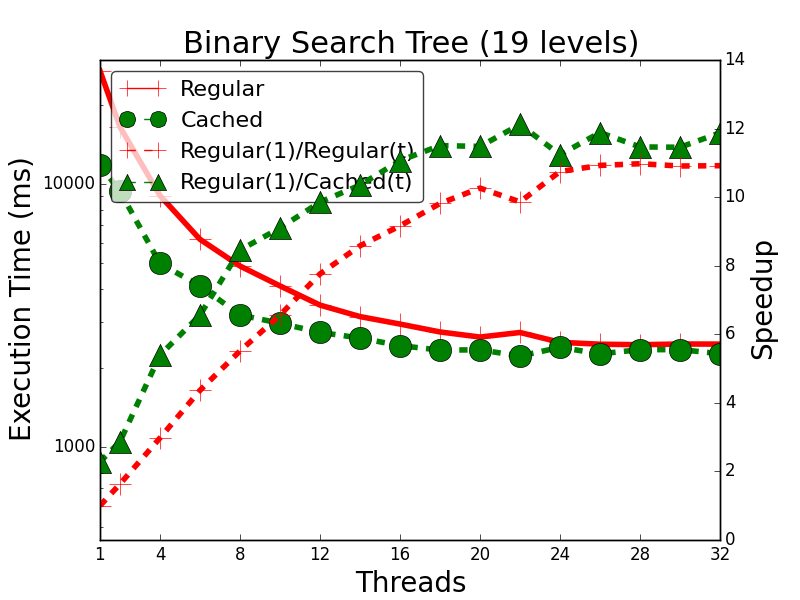
\includegraphics[width=\textwidth]{experiments/threads/cmp-key-value-19-ten.png}
           \label{fig:threads:key_value_19}
        \end{subfigure}
        ~
        \begin{subfigure}[b]{\plotsize\textwidth}
           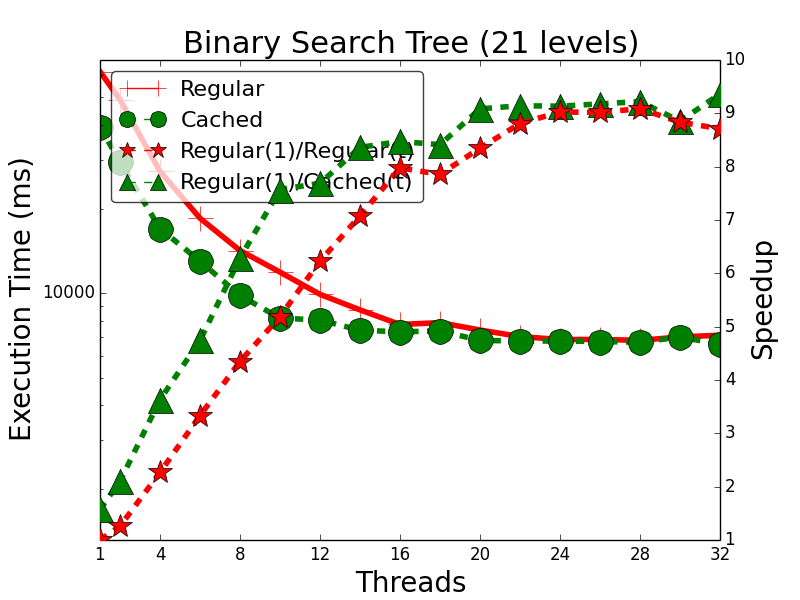
\includegraphics[width=\textwidth]{experiments/threads/cmp-key-value-21-ten.png}
           \label{fig:threads:key_value_21}
        \end{subfigure} \\

        \caption{Scalability for the Binary Search Tree program when using
        thread based facts.}

        \label{fig:threads:results_key_value}
\end{figure}

\clearpage
